\documentclass[oneside,a4paper,11pt,explicit]{book}
\usepackage[utf8]{inputenc}
\usepackage{../common/kultem}
\usepackage[english]{babel}

%% INSERT YOUR PACKAGES HERE
\usepackage[accsupp]{axessibility}  % improves PDF readability for those with disabilities.
\usepackage[hidelinks]{hyperref}
\usepackage{lipsum}
\usepackage{listings}
\usepackage{neuralnetwork}
\usepackage{pgfplots}
\pgfplotsset{compat=1.18}
\usetikzlibrary{arrows.meta, positioning, calc, decorations.pathreplacing, shapes.geometric, fit}
\usepackage{amsmath,amssymb}
\usepackage{tcolorbox}
\tcbuselibrary{skins,breakable}
\newtcolorbox{insightbox}[1][]{
    colback=blue!3, colframe=blue!40!black, fonttitle=\bfseries,
    title={Theoretical Insight}, #1
}

% Python typesetting
\usepackage{listings}
\lstset{language=Python,basicstyle=\ttm}

\hypersetup{
	colorlinks=true,
	linkcolor=cyan,
	filecolor=magenta,
	urlcolor=cyan,
}
\usepackage{wrapfig}
\usepackage[giveninits=true,sorting=none]{biblatex} %Imports biblatex package
\addbibresource{references.bib} %Import the bibliography file

% Custom commands used later
\newcommand{\ANNta}[2]{% 1: TA name ; 2: TA mail
	\href{mailto:#2}{\color{black}{#1}}%
}
\newcommand{\ANNsession}[1]{% 1: Session number
	\title{\ANNtitle}
	\subtitle{\ANNsubtitle{#1}}
	\author{\ANNprof}
	\assistants{\ANNtas{}}
	\date{\ANNyear{}}
	\setcounter{chapter}{#1}
	\addtocounter{chapter}{-1}
}
\newcommand{\ANNtopic}[1]{% 1: Session topic
	\maketitle%
	\chapter{#1}%
}

% General configuration, shared across sessions
\newcommand{\ANNtitle}{Artificial Neural Networks \& Deep Learning}
\newcommand{\ANNsubtitle}[1]{Exercise Session #1}
\newcommand{\ANNprof}{Prof. Dr. ir. Johan A. K. Suykens}
\newcommand{\ANNtas}{%
	\ANNta{Sonny Achten}{sonny.achten@kuleuven.be}\\ %
	% \ANNta{Bram De Cooman}{bram.decooman@kuleuven.be}\\ %
	\ANNta{Maung Thant}{thant.maung@student.kuleuven.be}\\ %
	\ANNta{Xinjie Zeng}{xzeng@esat.kuleuven.be}%
}
\newcommand{\ANNyear}{2024-2025}

\addto\captionsenglish{\renewcommand{\chaptername}{Session}}


\ANNsession{2}

\begin{document}

\ANNtopic{Recurrent Neural Networks}

\kulbox{{\noindent{\bf Note:}
There is no need to repeat the information provided during the guided session.
Answer the questions as concise and accurate as possible.
Show your understanding of the concepts and methods by linking your observations to the theory.
Use graphical and/or tabular presentations where needed.
The \textit{page limit} for this exercise is \textit{4 printed pages}, including figures.}}

This assignment focuses on recurrent neural networks and their applications as associative memory for pattern denoising or recognition, and as nonlinear autoregressive models for time-series prediction. 
For the former application, we study the Hopfield network, which is tested on a dataset of noisy handwritten digits.
The latter application is demonstrated on a dataset of chaotic laser data, where we use multi-layer perceptrons and long short-term memory networks to predict the continuation of the time series.

\section{Hopfield Network}

\begin{minipage}[t][][t]{0.75\textwidth}
A Hopfield network \cite{Hopfield, HopfieldCont} has one layer of $N$ neurons and is a fully interconnected recurrent neural network: each neuron is connected to every other neuron.
After initialization of all neurons (the initial input), the network is let to evolve: an output at time $t$ becomes an input at time $t+1$.
Thus to generate a series of outputs, we have to provide only one initial input.
In the course of this dynamical evolution the network should reach a stable state (an attractor), which is a configuration of neuron values that is not changed by subsequent updates of the network.
Networks of this kind are used as models of associative memory.
After initialization the network should evolve to the closest attractor.
\end{minipage}~\hspace{.5em}
\begin{minipage}[t][][c]{0.2\textwidth}
    \centering
    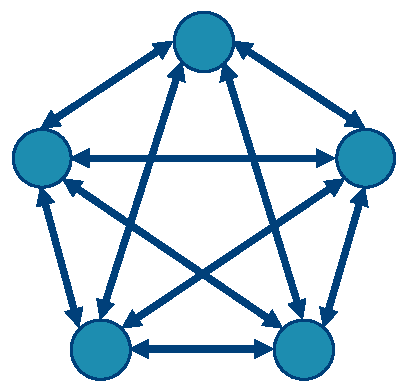
\includegraphics[width=\textwidth]{images/hop.pdf}
\end{minipage}

\kulbox{To answer the questions in this section, you will need the notebook \texttt{hopfield.ipynb} that you can find on toledo, or alternatively using \href{https://colab.research.google.com/github/psanchezML/KUL_ANNDL_ExerciseSessions/blob/main/session2/hopfield.ipynb}{this colab link}.}

%% ===================================================================
%%  THEORETICAL BACKGROUND
%% ===================================================================
\subsection*{Theoretical Background}

\subsubsection*{Energy Function and Dynamics}

The behaviour of a Hopfield network is governed by an \emph{energy function} (also called Lyapunov function).
For binary neurons with states $s_i \in \{-1, +1\}$ and symmetric weights ($w_{ij} = w_{ji}$, $w_{ii}=0$) the energy is
\begin{equation}\label{eq:hop-energy}
    E(\mathbf{s}) \;=\; -\frac{1}{2}\,\mathbf{s}^{\!\top} W\, \mathbf{s} \;-\; \mathbf{b}^{\!\top}\mathbf{s}\,,
\end{equation}
where $W\in\mathbb{R}^{N\times N}$ is the weight matrix and $\mathbf{b}$ is a bias vector.
A fundamental property is that this energy \emph{never increases} during an asynchronous update.
Thus the network always converges to a local minimum of~\eqref{eq:hop-energy}, which corresponds to a stored pattern (or a spurious state).

\begin{insightbox}
The energy landscape can be visualised as a hilly terrain: each stored pattern sits at the bottom of a \textbf{basin of attraction}.
When a (possibly noisy) input is presented, the network ``rolls downhill'' until it settles in the nearest basin, thereby recovering the closest stored pattern.
The deeper and wider the basin, the more robust the recall.
\end{insightbox}

\subsubsection*{Update Rules}

Two update strategies exist:
\begin{itemize}
    \item \textbf{Synchronous}: all neurons are updated simultaneously. Fast but may lead to oscillations in some networks.
    \item \textbf{Asynchronous}: one neuron is updated at a time (randomly selected). Guaranteed energy decrease at every step, hence guaranteed convergence for symmetric weights.
\end{itemize}

% --- TikZ figure: energy landscape schematic ---
\begin{figure}[h]
\centering
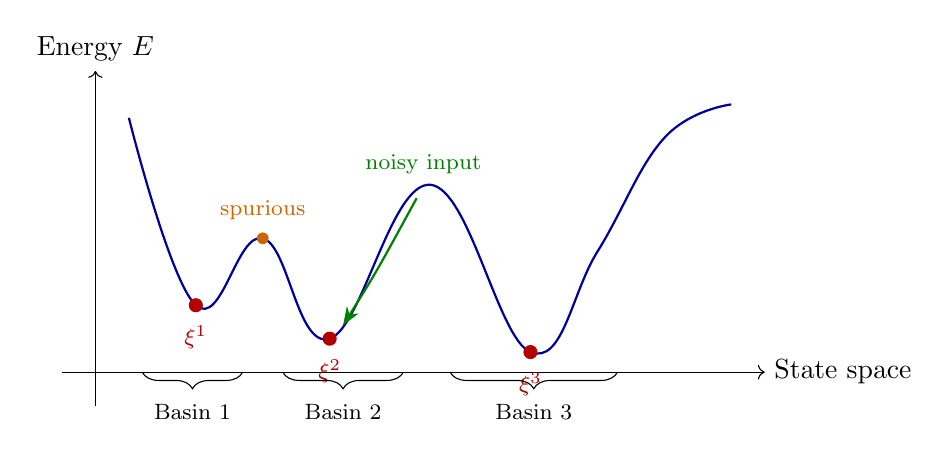
\begin{tikzpicture}[scale=0.85]
    \draw[->] (-0.5,0) -- (10,0) node[right] {State space};
    \draw[->] (0,-0.5) -- (0,4.5) node[above] {Energy $E$};
    \draw[thick, blue!60!black, smooth, tension=0.7]
        plot coordinates {(0.5,3.8) (1.5,1.0) (2.5,2.0) (3.5,0.5) (5.0,2.8) (6.5,0.3) (7.5,1.8) (8.5,3.5) (9.5,4.0)};
    \fill[red!70!black] (1.5,1.0) circle (3pt) node[below=4pt] {\footnotesize $\xi^1$};
    \fill[red!70!black] (3.5,0.5) circle (3pt) node[below=4pt] {\footnotesize $\xi^2$};
    \fill[red!70!black] (6.5,0.3) circle (3pt) node[below=4pt] {\footnotesize $\xi^3$};
    \fill[orange!80!black] (2.5,2.0) circle (2.5pt) node[above=3pt] {\footnotesize spurious};
    \draw[-{Stealth}, thick, green!50!black] (4.8,2.6) .. controls (4.2,1.5) .. (3.7,0.7);
    \node[green!50!black] at (4.9,3.1) {\footnotesize noisy input};
    \draw[decorate, decoration={brace, amplitude=6pt, mirror}] (0.7,0) -- (2.2,0)
        node[midway, below=8pt, font=\footnotesize] {Basin 1};
    \draw[decorate, decoration={brace, amplitude=6pt, mirror}] (2.8,0) -- (4.6,0)
        node[midway, below=8pt, font=\footnotesize] {Basin 2};
    \draw[decorate, decoration={brace, amplitude=6pt, mirror}] (5.3,0) -- (7.8,0)
        node[midway, below=8pt, font=\footnotesize] {Basin 3};
\end{tikzpicture}
\caption{Schematic energy landscape of a Hopfield network with three stored patterns $\xi^1,\xi^2,\xi^3$.  A noisy input (green arrow) converges to the nearest basin.  The local maximum between basins~1 and~2 is a spurious attractor.}
\label{fig:energy-landscape}
\end{figure}

\subsubsection*{Storage Capacity}

The \textbf{Hebbian learning rule} stores $T$ patterns of dimension $N$ via the outer-product rule:
\begin{equation}
    W = \frac{1}{T\,N}\sum_{\mu=1}^{T} \boldsymbol\xi^{\mu}\,(\boldsymbol\xi^{\mu})^{\!\top}, \qquad w_{ii}=0.
\end{equation}
A classical result \cite{Hopfield} shows that reliable retrieval is only possible when
\begin{equation}\label{eq:capacity}
    T \;\lesssim\; 0.14\,N\,.
\end{equation}
Beyond this capacity, \textbf{spurious attractors} emerge---stable states that are not stored patterns.
These include mixture states (superpositions of stored patterns) and negations of stored patterns.
The LSSM algorithm (used by MATLAB's \texttt{newhop}) can improve storage beyond this bound by using a more sophisticated weight calculation.

\kulbox{Explore the Hopfield network interactively with the \textbf{Hopfield Basin Explorer} demo app in \texttt{demos/hopfield\_basin\_explorer/}.  It visualises the energy landscape, basins of attraction, and digit reconstruction in 3D.  Run with: \texttt{streamlit run demos/hopfield\_basin\_explorer/app.py}}

%% ===================================================================
%%  EXERCISES
%% ===================================================================
\subsection*{Exercises}
\begin{questions}
    \item Create a Hopfield network with target patterns $[1, 1]$, $[-1, -1]$ and $[1, -1]$ and the corresponding number of neurons.
    Simulate the state evolution for various input vectors (e.g. random points or points of high symmetry) and note down the obtained attractors after a sufficient number of iterations.
    Are the real attractors the same as those used to create the network?
    If not, why do we get these unwanted attractors?
    How many iterations does it typically take to reach the attractor?
    What can you say about the stability of the attractors?

    \item Do the same for a three neuron Hopfield network, this time for the target patterns $[1, 1, 1]$, $[-1, -1, 1]$ and $[1, -1, -1]$.
    Use the analysis tools demonstrated in Exercise~1 (energy landscape, basins, fixed-point classification) to answer the following:
    \begin{itemize}
        \item Are all three target patterns stable fixed points?  If not, which ones are unstable and why?
        \item Visualise the energy landscape slices (at neuron~3 $= -1, 0, +1$).  Where are the energy minima relative to the stored patterns?
        \item Compare the basins of attraction under \textbf{synchronous} vs.\ \textbf{asynchronous} update.  Do the basins differ in shape or size?
        \item Can you find any \textbf{spurious attractors}?  Where do they sit in the 3D state space relative to the stored patterns?
        \item What happens when you start from the origin $[0, 0, 0]$?  Is the outcome deterministic?
    \end{itemize}

    \item Create a higher dimensional Hopfield network which has as attractors the handwritten digits from $0$ to $9$.
    Test the ability of the network to correctly retrieve these patterns when some noisy digits are given as input to the network.
    Try to answer the below questions by playing with these two parameters:
    \begin{itemize}
        \item \texttt{noise\_level} represents the level of noise that will corrupt the digits and is a positive number.
        \item \texttt{num\_iter} is the number of iterations the Hopfield network (having as input the noisy digits) will run.
    \end{itemize}
    Is the Hopfield model always able to reconstruct the noisy digits? If not why?
    What is the influence of the noise on the number of iterations?

    %% --- NEW EXERCISES ---
    \item \textbf{Capacity and Spurious States.}\;
    Systematically increase the number of stored \emph{random} binary patterns for a fixed network size (e.g.\ $N{=}100$).
    For each number of patterns, measure the fraction of patterns that are successfully retrieved after a fixed number of iterations.
    Plot the \emph{retrieval success rate} as a function of the number of stored patterns.
    \begin{itemize}
        \item Identify the experimental capacity threshold and compare it with the theoretical bound $\approx 0.14\,N$ from Eq.~\eqref{eq:capacity}.
        \item Characterise the spurious attractors you find beyond capacity: are they negations of stored patterns, mixture states, or something else?
    \end{itemize}
    Use the \texttt{capacity\_test} and \texttt{find\_spurious\_attractors} methods of the enhanced \texttt{HopfieldNetwork} class.

    \item \textbf{Basins of Attraction Analysis.}\;
    For the 3D Hopfield network from Exercise~2, exhaustively sample the state space (all $2^3 = 8$ binary vertices plus a dense continuous grid in $[-1,1]^3$) and classify each initial state by which attractor it converges to.
    \begin{itemize}
        \item Visualise the basins of attraction using the \texttt{plot\_basins} method.
              Use both the energy landscape (\texttt{plot\_energy\_landscape}) and the basin plot to identify which stored patterns are true attractors and which initial conditions lead to spurious states.
        \item Investigate whether changing from synchronous to asynchronous update affects the basin boundaries.
        \item Discuss the stability of each stored pattern: is every target pattern a genuine attractor?
    \end{itemize}
\end{questions}

%% ===================================================================
%%  MODERN HOPFIELD NETWORKS  (theory only)
%% ===================================================================
\subsection*{Modern Hopfield Networks and the Connection to Self-Attention}

Classical Hopfield networks use a quadratic energy function and binary states, leading to a storage capacity that scales only \emph{linearly} with the network dimension ($\sim 0.14\,N$).
\textbf{Modern Hopfield Networks} \cite{ModernHopfield} replace the quadratic energy with an exponential interaction, dramatically increasing the capacity to \emph{exponential} in the pattern dimension~$d$.

\subsubsection*{Energy and Update Rule}

Given $T$ stored patterns $\boldsymbol\xi^1,\dots,\boldsymbol\xi^T \in \mathbb{R}^d$ and a query (state) $\boldsymbol\xi \in \mathbb{R}^d$, the modern continuous energy is
\begin{equation}\label{eq:modern-energy}
    E(\boldsymbol\xi) \;=\; -\mathrm{lse}\!\bigl(\beta,\, X^{\!\top}\boldsymbol\xi\bigr) \;+\; \tfrac{1}{2}\,\boldsymbol\xi^{\!\top}\boldsymbol\xi \;+\; \text{const},
\end{equation}
where $X = [\boldsymbol\xi^1 \!\mid\! \cdots \!\mid\! \boldsymbol\xi^T]$ stacks the stored patterns as columns, $\mathrm{lse}(\beta, \mathbf{z}) = \beta^{-1}\log\!\bigl(\sum_i e^{\beta z_i}\bigr)$ is the log-sum-exp, and $\beta > 0$ is an inverse temperature.
The corresponding update rule is
\begin{equation}\label{eq:modern-update}
    \boldsymbol\xi^{\mathrm{new}} \;=\; X\,\mathrm{softmax}\!\bigl(\beta\, X^{\!\top}\boldsymbol\xi\bigr).
\end{equation}

\subsubsection*{Equivalence to Transformer Self-Attention}

The update~\eqref{eq:modern-update} is \emph{mathematically equivalent} to one step of Transformer self-attention \cite{Attention}.
The mapping is:

\begin{center}
\renewcommand{\arraystretch}{1.3}
\begin{tabular}{l@{\qquad$\longleftrightarrow$\qquad}l}
    \textbf{Modern Hopfield} & \textbf{Self-Attention} \\
    \hline
    Stored patterns $X$ (Keys) & Key matrix $K$ \\
    State pattern $\boldsymbol\xi$ (Query) & Query vector $Q$ \\
    Pattern projections $X$ (Values) & Value matrix $V$ \\
    $\beta = 1/\sqrt{d_k}$ & Attention scaling \\
    Update: $X\,\mathrm{softmax}(\beta X^{\!\top}\boldsymbol\xi)$ & Attention: $V\,\mathrm{softmax}(Q K^{\!\top}/\sqrt{d_k})$ \\
\end{tabular}
\end{center}

\begin{insightbox}
Transformer self-attention can be interpreted as a \textbf{single retrieval step of a modern Hopfield network}: the query attends to keys (stored patterns) and retrieves a weighted combination of values.
The inverse temperature $\beta$ controls the sharpness of retrieval---large $\beta$ yields one-hot attention (nearest-neighbour lookup), while small $\beta$ yields a soft average.
This unifying view reveals that attention mechanisms in large language models are performing \emph{associative memory retrieval} at every layer.
\end{insightbox}

% --- TikZ figure: Modern Hopfield ↔ Self-Attention ---
\begin{figure}[h]
\centering
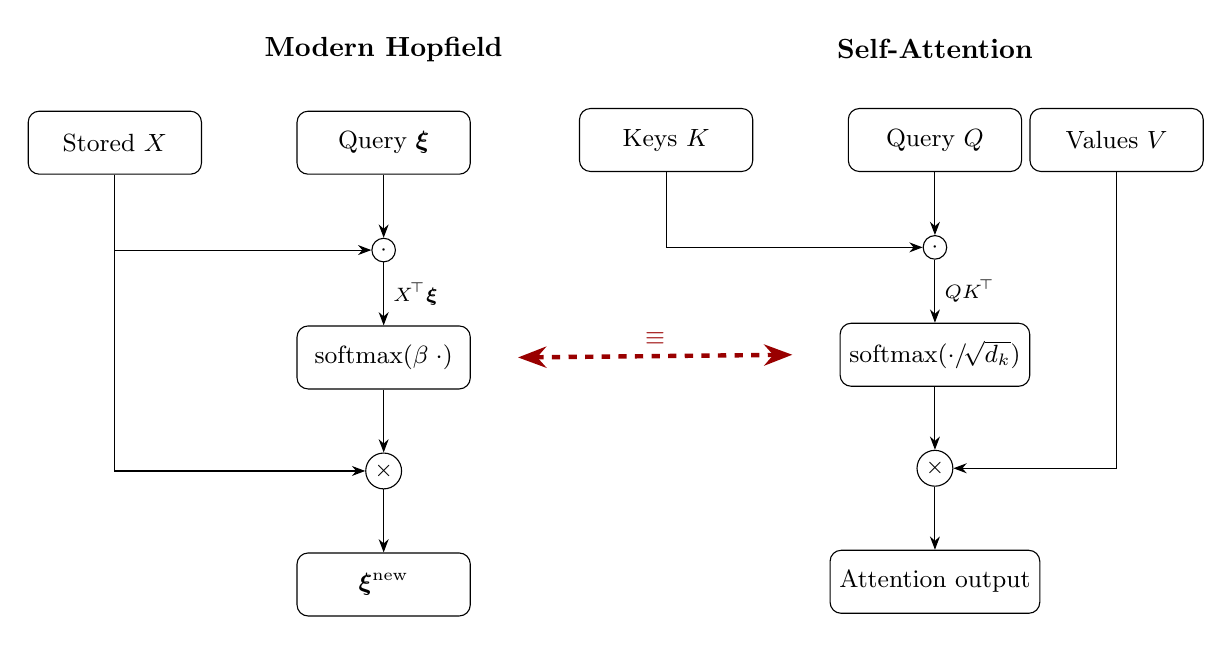
\begin{tikzpicture}[
    >=Stealth, node distance=8mm,
    block/.style={draw, rounded corners, minimum width=22mm, minimum height=8mm, align=center, font=\small},
    op/.style={draw, circle, inner sep=1.5pt, font=\footnotesize},
]
    % Modern Hopfield side
    \node[font=\bfseries] (mh_title) {Modern Hopfield};
    \node[block, below=5mm of mh_title] (xi) {Query $\boldsymbol\xi$};
    \node[block, left=12mm of xi] (X) {Stored $X$};
    \node[op, below=8mm of xi] (dot1) {$\cdot$};
    \node[block, below=8mm of dot1] (sm1) {$\mathrm{softmax}(\beta\;\cdot)$};
    \node[op, below=8mm of sm1] (dot2) {$\times$};
    \node[block, below=8mm of dot2] (out1) {$\boldsymbol\xi^{\mathrm{new}}$};

    \draw[->] (xi) -- (dot1);
    \draw[->] (X) |- (dot1);
    \draw[->] (dot1) -- node[right, font=\scriptsize]{$X^{\!\top}\boldsymbol\xi$} (sm1);
    \draw[->] (sm1) -- (dot2);
    \draw[->] (X) |- (dot2);
    \draw[->] (dot2) -- (out1);

    % Self-Attention side
    \node[font=\bfseries, right=40mm of mh_title] (sa_title) {Self-Attention};
    \node[block, below=5mm of sa_title] (Q) {Query $Q$};
    \node[block, left=12mm of Q] (K) {Keys $K$};
    \node[op, below=8mm of Q] (dot3) {$\cdot$};
    \node[block, below=8mm of dot3] (sm2) {$\mathrm{softmax}(\cdot/\!\sqrt{d_k})$};
    \node[op, below=8mm of sm2] (dot4) {$\times$};
    \node[block, right=12mm of K] (V) at (K -| sa_title) {Values $V$};
    \node[block, below=8mm of dot4] (out2) {Attention output};

    \draw[->] (Q) -- (dot3);
    \draw[->] (K) |- (dot3);
    \draw[->] (dot3) -- node[right, font=\scriptsize]{$QK^{\!\top}$} (sm2);
    \draw[->] (sm2) -- (dot4);
    \draw[->] (V) |- (dot4);
    \draw[->] (dot4) -- (out2);

    % Equivalence arrow
    \draw[<->, ultra thick, red!60!black, dashed] ([xshift=6mm]sm1.east) -- ([xshift=-6mm]sm2.west) node[midway, above, font=\small\bfseries, red!60!black] {$\equiv$};
\end{tikzpicture}
\caption{The Modern Hopfield update (left) is structurally identical to Transformer self-attention (right).  Stored patterns play the role of Keys, the query state maps to the Query, and the retrieved output corresponds to the attention-weighted Values.}
\label{fig:modern-hopfield-attention}
\end{figure}

\subsubsection*{Exponential Storage Capacity}

While classical Hopfield networks can store at most $\sim 0.14\,N$ patterns, modern Hopfield networks achieve a capacity that is \emph{exponential} in the pattern dimension:
\begin{equation}
    T_{\max} \;\sim\; \exp\!\bigl(\alpha\, d\bigr), \qquad \alpha > 0.
\end{equation}
This exponential scaling is enabled by the log-sum-exp energy, which creates much sharper separation between stored patterns in the energy landscape.
Intuitively, the softmax creates a ``winner-take-all'' competition among stored patterns, allowing far more patterns to coexist without interference.

\kulbox{Explore the connection between Modern Hopfield Networks and self-attention with the interactive demo in \texttt{demos/modern\_hopfield\_attention/}. It lets you compare classical vs.\ modern retrieval, adjust the temperature $\beta$, and visualise how attention maps sharpen.
Run with: \texttt{streamlit run demos/modern\_hopfield\_attention/app.py}}


\section{Timeseries Prediction}

A time series is a sequence of observations, ordered in time.
Forecasting involves training a model on historical data and using them to predict future observations.
A simple example is a linear auto-regressive model.
The linear auto-regressive (AR) model of a time-series $Z_t$ with $t = 1,2,\dots,\infty$ is given by
\begin{equation*}
    \hat{z}_t = a_1 z_{t-1} + a_2 z_{t-2} + \dots + a_p z_{t-p} \enspace,
\end{equation*}
with $a_i \in \mathbb{R}$ for $i=1,\dots,p$ and $p$ the model lag.
The prediction for a certain time $t$ is equal to a weighted sum of the previous values up to a certain lag $p$.
In a similar way, the nonlinear variant (NAR) is described as
\begin{equation*}
    \hat{z}_t = f(z_{t-1},z_{t-2}, \dots,z_{t-p}) \enspace.
\end{equation*}

A depiction of this process can be found in Figure~\ref{fig:nar}.
Remark that in this way, the time-series identification can be written as a classical black-box regression modeling problem $\hat{y}_t = f(x_t)$, with $y_t = z_t$ and $x_t = [z_{t-1}, z_{t-2}, \dots, z_{t-p}]$.
When preparing the dataset and applying train/validation/test splits, it is important to prevent \emph{data leakage} by respecting the temporal information flow.
More precisely, a datapoint $z_t$ should not be part of two splits --- either as input $x_t$ or target $y_t$ --- and training (or validation) sets should not contain datapoints that occur after test datapoints.

\begin{figure}[h]
	\centering
	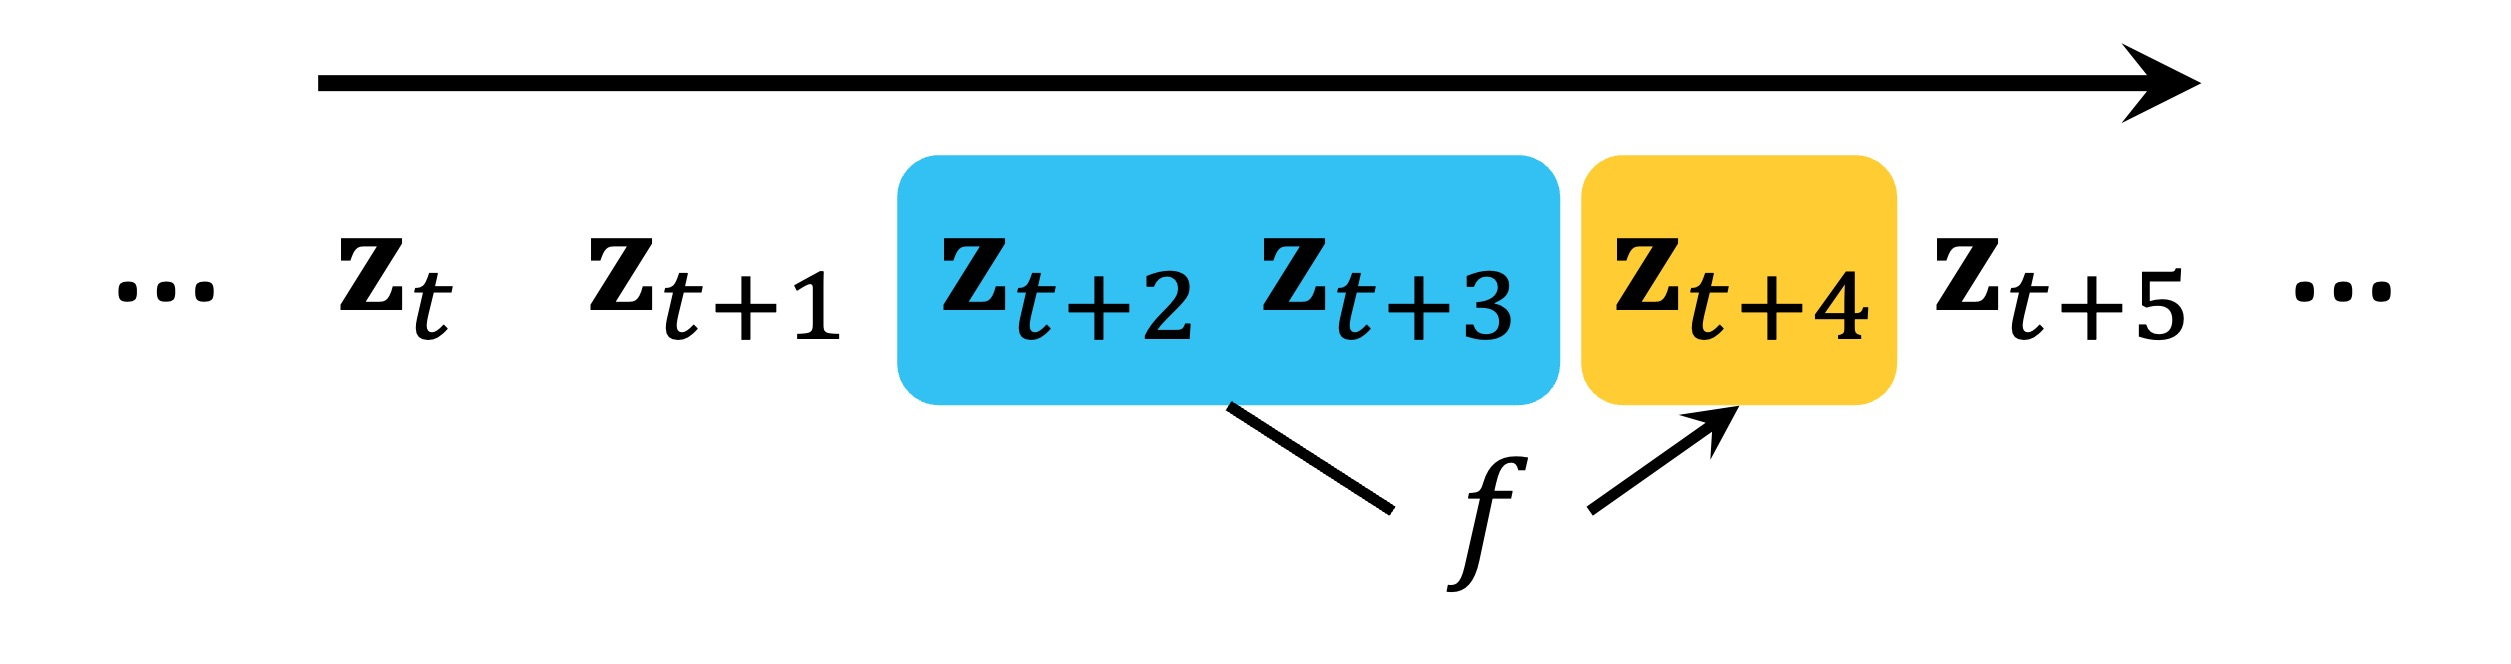
\includegraphics[width=0.6\textwidth]{images/nar.jpg}
	\caption{Schematic representation of the nonlinear auto-regressive model with lag $p=2$.}
	\label{fig:nar}
\end{figure}

\kulbox{To answer the questions in this section, you will need the notebook \texttt{time\_series.ipynb} that you can find on toledo, or alternatively using \href{https://colab.research.google.com/github/psanchezML/KUL_ANNDL_ExerciseSessions/blob/main/session2/time_series.ipynb}{this colab link}.}

%% ===================================================================
%%  ARCHITECTURE THEORY
%% ===================================================================

\subsection*{Recurrent Neural Networks (RNNs)}

A recurrent neural network \cite{Elman1990} processes a sequence element-by-element, maintaining a hidden state $\mathbf{h}_t$ that summarises all previously seen inputs:
\begin{align}
    \mathbf{h}_t &= \tanh\!\bigl(W_h\,\mathbf{h}_{t-1} + W_x\,\mathbf{x}_t + \mathbf{b}_h\bigr), \label{eq:rnn-hidden}\\
    \hat{y}_t &= W_y\,\mathbf{h}_t + b_y. \label{eq:rnn-output}
\end{align}
The key feature is \textbf{weight sharing}: the same matrices $W_h$, $W_x$ are applied at every time step, giving the model a strong inductive bias toward \emph{sequential processing} with translational equivariance in time.

% --- TikZ: unfolded RNN ---
\begin{figure}[h]
\centering
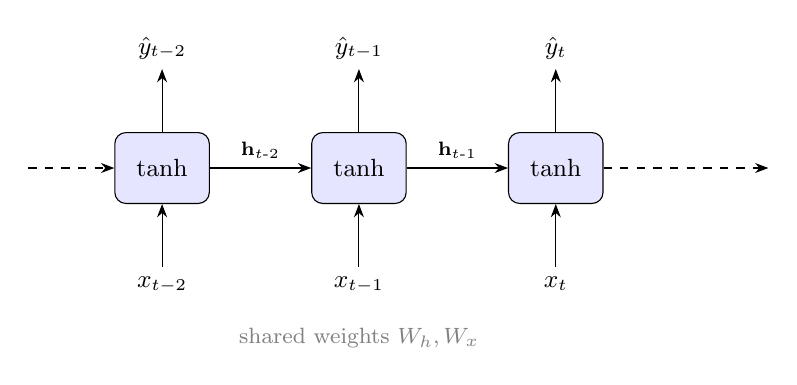
\begin{tikzpicture}[
    >=Stealth, node distance=14mm,
    cell/.style={draw, rounded corners, minimum width=12mm, minimum height=9mm, fill=blue!10, font=\small},
    io/.style={font=\small},
]
    \foreach \i in {1,2,3} {
        \node[cell] (h\i) at (2.5*\i, 0) {$\tanh$};
        \node[io, below=8mm of h\i] (x\i) {$x_{t\ifnum\i=1{-2}\fi\ifnum\i=2{-1}\fi\ifnum\i=3{}\fi}$};
        \node[io, above=8mm of h\i] (y\i) {$\hat{y}_{t\ifnum\i=1{-2}\fi\ifnum\i=2{-1}\fi\ifnum\i=3{}\fi}$};
        \draw[->] (x\i) -- (h\i);
        \draw[->] (h\i) -- (y\i);
    }
    \draw[->] (h1) -- node[above, font=\scriptsize]{$\mathbf{h}_{t\text{-}2}$} (h2);
    \draw[->] (h2) -- node[above, font=\scriptsize]{$\mathbf{h}_{t\text{-}1}$} (h3);
    \draw[->, dashed] (0.8,0) -- (h1);
    \draw[->, dashed] (h3) -- (10.2,0);
    \node[below=2mm of x2, font=\footnotesize, gray] {shared weights $W_h, W_x$};
\end{tikzpicture}
\caption{An RNN unfolded over three time steps. The same weights are reused at every step; the hidden state $\mathbf{h}_t$ carries temporal information forward.}
\label{fig:rnn-unfolded}
\end{figure}

\begin{insightbox}[title={The Vanishing Gradient Problem}]
During backpropagation through time (BPTT), gradients are multiplied by $W_h$ at each step.
If the spectral radius of $W_h$ is less than 1, gradients \emph{vanish} exponentially with sequence length; if greater than 1, they \emph{explode} \cite{VanishingGradient}.
This limits simple RNNs to learning dependencies over \textbf{short-to-moderate} time horizons.
\end{insightbox}

\subsection*{Long Short-Term Memory Network (LSTM)}

Long Short Term Memory networks \cite{LSTM} solve the vanishing gradient problem by introducing a \emph{cell state} $\mathbf{c}_t$ and three \emph{gates} that regulate information flow:
\begin{align}
    \mathbf{f}_t &= \sigma\!\bigl(W_f\,[\mathbf{h}_{t-1};\,\mathbf{x}_t] + \mathbf{b}_f\bigr) & &\text{(forget gate)} \label{eq:lstm-forget}\\
    \mathbf{i}_t &= \sigma\!\bigl(W_i\,[\mathbf{h}_{t-1};\,\mathbf{x}_t] + \mathbf{b}_i\bigr) & &\text{(input gate)} \label{eq:lstm-input}\\
    \tilde{\mathbf{c}}_t &= \tanh\!\bigl(W_c\,[\mathbf{h}_{t-1};\,\mathbf{x}_t] + \mathbf{b}_c\bigr) & &\text{(candidate)} \\
    \mathbf{c}_t &= \mathbf{f}_t \odot \mathbf{c}_{t-1} \;+\; \mathbf{i}_t \odot \tilde{\mathbf{c}}_t & &\text{(cell update)} \label{eq:lstm-cell}\\
    \mathbf{o}_t &= \sigma\!\bigl(W_o\,[\mathbf{h}_{t-1};\,\mathbf{x}_t] + \mathbf{b}_o\bigr) & &\text{(output gate)} \\
    \mathbf{h}_t &= \mathbf{o}_t \odot \tanh(\mathbf{c}_t) & &\text{(hidden state)} \label{eq:lstm-hidden}
\end{align}
where $\sigma$ is the sigmoid function, $\odot$ denotes element-wise multiplication, and $[\cdot\,;\,\cdot]$ is concatenation.

The cell state acts as a \textbf{conveyor belt}: the forget gate decides what to discard, the input gate decides what new information to write, and the output gate controls what to expose.
Because the cell state is updated via \emph{additive} interactions (Eq.~\ref{eq:lstm-cell}), gradients can flow across many time steps without vanishing, enabling LSTMs to capture \textbf{long-range dependencies}.

% --- TikZ: LSTM cell ---
\begin{figure}[h]
\centering
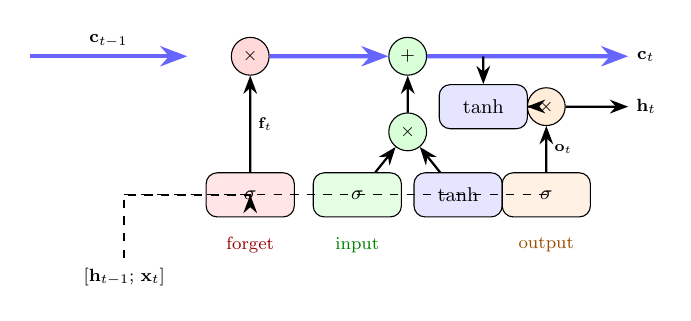
\begin{tikzpicture}[
    >=Stealth, scale=0.8, every node/.style={scale=0.8},
    gate/.style={draw, circle, inner sep=2pt, minimum size=7mm, font=\small},
    op/.style={draw, circle, inner sep=1pt, minimum size=6mm, font=\footnotesize},
    arr/.style={->, thick},
    block/.style={draw, rounded corners, minimum width=14mm, minimum height=7mm, fill=yellow!15, font=\small},
]
    % Cell state line
    \draw[arr, line width=1.5pt, blue!60] (-1,3) -- node[above, font=\footnotesize, black]{$\mathbf{c}_{t-1}$} (1.5,3);
    \node[op, fill=red!15] (forget) at (2.5,3) {$\times$};
    \node[op, fill=green!15] (add) at (5,3) {$+$};
    \draw[arr, line width=1.5pt, blue!60] (forget) -- (add);
    \draw[arr, line width=1.5pt, blue!60] (add) -- (8.5,3) node[right, black, font=\footnotesize]{$\mathbf{c}_t$};

    % Forget gate
    \node[block, fill=red!10] (fg) at (2.5,0.8) {$\sigma$};
    \draw[arr] (fg) -- node[right, font=\scriptsize]{$\mathbf{f}_t$} (forget);
    \node[font=\footnotesize, red!60!black] at (2.5,0) {forget};

    % Input gate + candidate
    \node[block, fill=green!10] (ig) at (4.2,0.8) {$\sigma$};
    \node[block, fill=blue!10] (cand) at (5.8,0.8) {$\tanh$};
    \node[op, fill=green!15] (imul) at (5,1.8) {$\times$};
    \draw[arr] (ig) -- (imul);
    \draw[arr] (cand) -- (imul);
    \draw[arr] (imul) -- (add);
    \node[font=\footnotesize, green!50!black] at (4.2,0) {input};

    % Output gate
    \node[block, fill=orange!10] (og) at (7.2,0.8) {$\sigma$};
    \node[op, fill=orange!15] (omul) at (7.2,2.2) {$\times$};
    \node[block, fill=blue!10] (otanh) at (6.2,2.2) {$\tanh$};
    \draw[arr] (og) -- node[right, font=\scriptsize]{$\mathbf{o}_t$} (omul);
    \draw[arr] (6.2,3) -- (otanh);
    \draw[arr] (otanh) -- (omul);
    \draw[arr] (omul) -- (8.5,2.2) node[right, font=\footnotesize]{$\mathbf{h}_t$};
    \node[font=\footnotesize, orange!60!black] at (7.2,0) {output};

    % Inputs
    \node[font=\footnotesize] at (0.5,-0.5) {$[\mathbf{h}_{t-1};\,\mathbf{x}_t]$};
    \draw[arr, dashed] (0.5,-0.2) -- (0.5,0.8) -| (fg);
    \draw[dashed] (0.5,0.8) -| (ig);
    \draw[dashed] (0.5,0.8) -| (cand);
    \draw[dashed] (0.5,0.8) -| (og);
\end{tikzpicture}
\caption{LSTM cell architecture.  The cell state $\mathbf{c}_t$ (blue line) flows left to right, modulated by the forget gate ($\times$, red) and enriched by the input gate ($+$, green).  The output gate (orange) controls the exposed hidden state.}
\label{fig:lstm-cell}
\end{figure}


\subsection*{Multilayer Perceptron for Time Series}

The MLP treats time-series prediction as a \emph{static regression} problem.
The input is a fixed window of $p$ past values $[z_{t-1}, \dots, z_{t-p}]$ and the output is the prediction $\hat{z}_t$.
The training is done in feedforward mode:
\begin{equation}
    \hat{z}_{t} = w^\top\tanh(V [z_{t-1} ; z_{t-2}; ...; z_{t-p}] + \beta).
\end{equation}
In order to make predictions, the trained network is used in an iterative way as a recurrent network:
\begin{equation}
    \hat{z}_{t} = w^\top\tanh(V [\hat{z}_{t-1} ; \hat{z}_{t-2}; ...; \hat{z}_{t-p}] + \beta).
\end{equation}

% --- TikZ: sliding window ---
\begin{figure}[h]
\centering
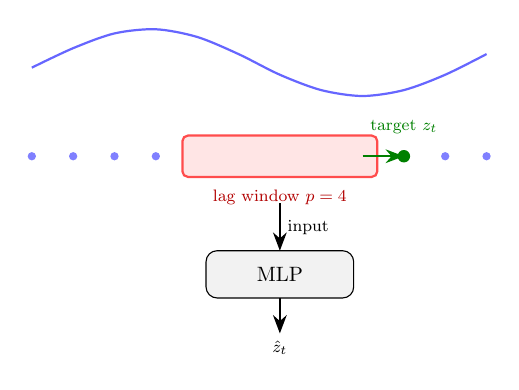
\begin{tikzpicture}[>=Stealth, scale=0.75, every node/.style={scale=0.75}]
    % Time series
    \foreach \i in {0,...,11} {
        \pgfmathsetmacro{\yv}{1.5+0.8*sin(40*\i)+0.3*cos(80*\i)}
        \fill[blue!50] (\i*0.7, 0) circle (2pt);
        \ifnum\i>0
            \pgfmathsetmacro{\yprev}{1.5+0.8*sin(40*(\i-1))+0.3*cos(80*(\i-1))}
        \fi
    }
    \draw[thick, blue!60, smooth] plot coordinates {
        (0,1.5) (0.7,1.83) (1.4,2.08) (2.1,2.15) (2.8,2.02) (3.5,1.73)
        (4.2,1.38) (4.9,1.12) (5.6,1.02) (6.3,1.12) (7.0,1.38) (7.7,1.73)
    };

    % Window
    \draw[thick, red!70, fill=red!10, rounded corners=2pt]
        (2.8-0.25,-0.35) rectangle (5.6+0.25,0.35);
    \node[below, red!70!black, font=\footnotesize] at (4.2,-0.45) {lag window $p=4$};

    % Target
    \draw[->, thick, green!50!black] (5.6,0) -- (6.3,0);
    \fill[green!50!black] (6.3,0) circle (3pt);
    \node[above, green!50!black, font=\footnotesize] at (6.3,0.25) {target $z_t$};

    % Arrow to MLP
    \draw[->, thick] (4.2,-0.8) -- (4.2,-1.6) node[midway, right, font=\footnotesize] {input};
    \node[draw, rounded corners, fill=gray!10, minimum width=25mm, minimum height=8mm] at (4.2,-2.0) {MLP};
    \draw[->, thick] (4.2,-2.4) -- (4.2,-3.0) node[below, font=\footnotesize] {$\hat{z}_t$};
\end{tikzpicture}
\caption{The MLP approach: a sliding window of $p$ past values is fed as a fixed-size input vector.  The temporal structure is encoded \emph{only} through the lag embedding.}
\label{fig:mlp-sliding-window}
\end{figure}

To format the timeseries for training, you can use the provided function \texttt{prepare\_timeseries}.
Make sure you understand what this function does by trying it out on a small toy example.
To make predictions, a \texttt{for} loop needs to be implemented that includes the predicted value from the previous timestep in the input vector to predict the next timestep.
As this is a stateful model, make sure to reset the internal state using the \texttt{reset\_states} function before making new predictions.

\subsection*{Inductive Biases of Sequential Models}

\begin{insightbox}[title={Why does architecture matter?}]
Different architectures impose different \emph{inductive biases}---implicit assumptions about the data:
\begin{itemize}
    \item \textbf{MLP}: assumes all relevant information is within a \emph{fixed window} of $p$ past values.  No notion of sequential order beyond position in the input vector.  Works best when the system has \textbf{strong local structure} and a well-defined lag.
    \item \textbf{Simple RNN}: assumes \emph{sequential processing} with shared weights at each step.  The hidden state carries a compressed summary of the past.  Excels at \textbf{moderate-range periodic} patterns but struggles with very long dependencies due to vanishing gradients.
    \item \textbf{LSTM}: adds \emph{selective memory} through gating.  Can learn to remember information over hundreds of steps.  Best suited for data with \textbf{long-range dependencies} that simpler models cannot capture.
\end{itemize}
Choosing the right architecture requires understanding the \emph{temporal structure} of your data---which is why exploratory data analysis (autocorrelation, spectral analysis) is so valuable before modelling.
\end{insightbox}


%% ===================================================================
%%  DATASETS
%% ===================================================================

\subsection*{Santa Fe Laser Dataset}
The Santa Fe laser dataset is obtained from a chaotic laser which can be described as a nonlinear dynamical system.
The first $1000$ data points can be used for training and validation purposes.
The aim is to predict the next $100$ points (it is forbidden to include these points in the training or validation sets!).
Both datasets are stored in \texttt{SantaFe.npz} and are shown in Figure~\ref{fig:santafe}.
Before training any of the models, it is important to normalize the data, such that it has zero mean and unit variance.

This dataset has \textbf{strong local nonlinear structure}: the value at time $t$ is largely determined by a short window of recent values.
An MLP with a well-chosen lag can capture this mapping directly and efficiently, without the overhead of sequential processing.

\begin{figure}[h]
	\centering
	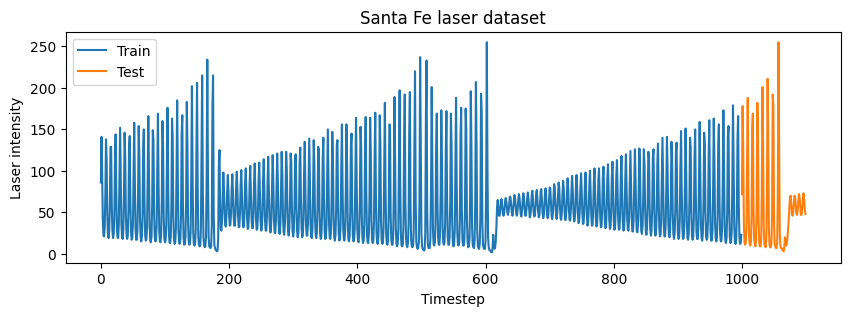
\includegraphics[width=0.9\textwidth]{images/santafe.png}
	\caption{Visualization of the Santa Fe laser dataset.}
	\label{fig:santafe}
\end{figure}

\subsection*{Mackey-Glass Time Series}
The Mackey-Glass equation \cite{MackeyGlass} is a delay differential equation originally proposed to model physiological control systems:
\begin{equation}
    \frac{dx}{dt} = \frac{\beta\, x(t-\tau)}{1 + x(t-\tau)^n} - \gamma\, x(t),
\end{equation}
with typical parameters $\beta=0.2$, $\gamma=0.1$, $n=10$.
The delay parameter $\tau$ controls the complexity: for $\tau > 17$ the system becomes chaotic.

With $\tau = 30$, the current value depends on information from \textbf{30 time steps in the past}, creating genuine long-range dependencies.
Simple RNNs suffer from vanishing gradients over these spans, making this the ideal dataset to demonstrate the advantage of \textbf{LSTMs}, whose gating mechanism can selectively preserve information across long horizons.

\subsection*{Sunspot Numbers}
Monthly sunspot counts have been recorded for over 300~years, making this one of the oldest scientific time series.
The data exhibits a prominent $\sim$11-year cycle (approximately 132~months) with varying amplitude and shape from cycle to cycle.

The regularity of the cycle means that the hidden state of a \textbf{simple RNN} can naturally track the phase of the oscillation, giving it an edge over MLPs (which would require an impractically large lag to see a full cycle) while not needing the heavy gating of an LSTM (since the relevant dependencies are moderate in length and the pattern is quasi-periodic).

\kulbox{Explore all three datasets interactively with the \textbf{Time Series Model Comparison} demo in \texttt{demos/timeseries\_explorer/}.
It provides EDA tools, side-by-side model training, and detailed ablation comparisons.
Run with: \texttt{streamlit run demos/timeseries\_explorer/app.py}}

%% ===================================================================
%%  EXERCISES
%% ===================================================================
\subsection*{Exercises}
\begin{questions}
    \item Train an MLP with one hidden layer on the \textbf{Santa Fe} dataset.
    Investigate the model performance with different lags and number of neurons.
    Discuss how the model looks and explain clearly how you tune the parameters and what the influence on the final prediction is.
    Which combination of parameters gives the best performance (MSE) on the test set?
	\item Do the same for the LSTM model and explain the design process.
    What is the effect of changing the lag value for the LSTM network?
	\item Compare the results of the recurrent MLP with the LSTM. Which model do you prefer and why?

    %% --- NEW EXERCISES ---
    \item \textbf{Ablation Study Across Datasets.}\;
    Train an MLP, a Simple RNN, and an LSTM on \emph{all three} datasets (Santa Fe, Mackey-Glass with $\tau{=}30$, Sunspot numbers).
    For each model--dataset pair:
    \begin{itemize}
        \item Report the test MSE and plot the predicted vs.\ actual time series.
        \item Create a summary table (3 models $\times$ 3 datasets).
        \item Discuss which model performs best on each dataset and \emph{why}, relating your observations to the inductive biases described above and to the data characteristics you discover in Exercise~5.
    \end{itemize}
    Ensure the comparison is fair: use the same lag, training budget, and validation strategy across models for each dataset.

    \item \textbf{Time Series EDA and Feature Analysis.}\;
    Before fitting any model, perform an exploratory data analysis on each of the three datasets:
    \begin{itemize}
        \item Plot the raw time series with rolling mean and standard deviation.
        \item Compute and plot the autocorrelation (ACF) and partial autocorrelation (PACF) functions.
        \item Estimate the spectral density to identify dominant frequencies.
        \item Run an Augmented Dickey-Fuller (ADF) test for stationarity.
    \end{itemize}
    Use the results to justify your choice of lag $p$ for each dataset and discuss what the ACF/PACF tell you about the nature of each time series (short-range vs.\ long-range dependencies, periodicity, trend).
\end{questions}


\section*{References}
\printbibliography[heading=none]

\end{document}
